\documentclass[12pt,a4paper]{article}

\input{/home/tabaka/Documents/GitHub/Defs/defs.tex}

\setcounter{zadaniaRozdzial}{3}

\begin{document}
	
	\begin{center}
		\LARGE Extra zadania - geometria
	\end{center}
	\vspace{1.5cm}
	
	\ZbiorZadanie{Na rysunku obok punkty $A,B,C$ należą do okręgu oraz $|AB|=|AC|$. Średnica $AD$ zawiera wysokość $AE$ trójkąta $ABC$. Wiedząc, że $|AE|=12\,\mathrm{cm}$ oraz $|ED|=3\,\mathrm{cm}$, oblicz długości boków tego trójkąta.
		
	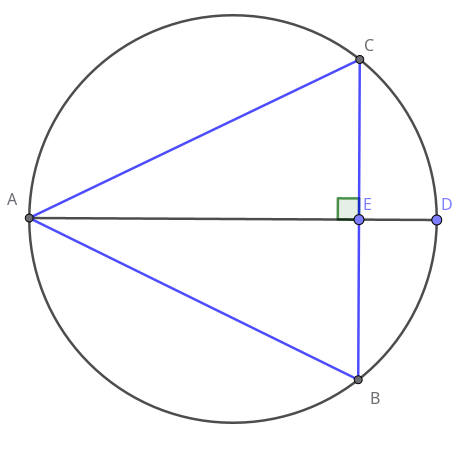
\includegraphics[scale=0.7]{ExK_1_2}}
	
	\ZbiorZadanie{Na rysunku obok boki $AB$ i $BC$ trójkąta $ABC$ są styczne do okręgu o środku w punkcie $O$, odpowiednio w punktach $D$ i $E$. Odległość punktu $C$ od punktu $O$ jest równa $5$. Punkty $C,O,D$ są współliniowe. Okrąg przecina bok $AC$ kolejno w punktach $P$ i $Q$. Wiedząc, że $|PQ|=|PC|=2\sqrt{2}$, oblicz:
		\begin{enumerate}[a)]
			\item promień okręgu,
			\item długości odcinków, na jakie punkt $E$ dzieli bok $BC$.
		\end{enumerate}
		
		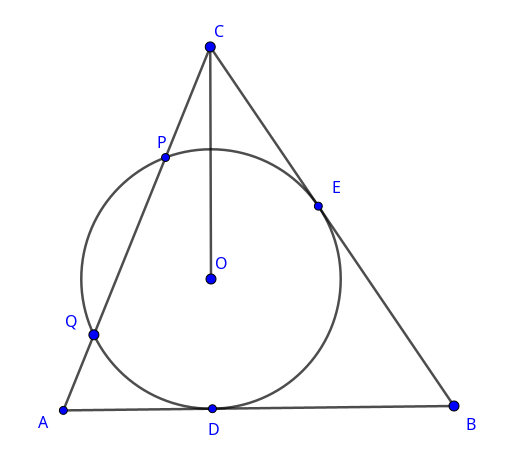
\includegraphics[scale=0.7]{ExK_1_3}}
		
	\ZbiorZadanie{Wysokość trójkąta równobocznego jest o $3\,\mathrm{cm}$ dłuższa od promienia okręgu opisanego na tym trójkącie. Oblicz długość boku trójkąta.}
	
	\ZbiorZadanie{Cięciwa $CD$ okręgu jest równoległa do średnicy $AB$. Wykaż, że różnica miar kątów $ACD$ i $CDA$ jest równa $90^\circ$.}
	
	\ZbiorZadanie{Promień okręgu opisanego na trójkącie prostokątnym jest równy $6\,\mathrm{cm}$. Oblicz odległość środka ciężkości tego trójkąta od wierzchołka kąta prostego.}
	
	\ZbiorZadanie{W trójkącie prostokątnym jedna z przyprostokątnych ma długość $65\,\mathrm{cm}$, a wysokość poprowadzona z wierzchołka kąta prostego jest równa $60\,\mathrm{cm}$. Oblicz promień okręgu opisanego na tym trójkącie.}
	
	\ZbiorZadanie{W okręgu poprowadzono dwie cięciwy $AB$ i $CD$, które przecięły się w punkcie $P$. Wiedząc, że $|AP|=10\,\mathrm{cm}$, $|BP|=4\,\mathrm{cm}$ oraz $|PD|=2{,}5\,\mathrm{cm}$, oblicz $|CP|$.}
	
	\ZbiorZadanie{Punkt $P$ przecięcia cięciw $AB$ i $CD$ okręgu dzieli cięciwę $AB$ na odcinki długości $8\,\mathrm{cm}$ i $3\,\mathrm{cm}$. Wiedząc, że $|CP|:|PD|=3:2$, oblicz długość cięciwy $CD$.}
	
	\ZbiorZadanie{Punkty $A,B,C$ należą do okręgu. Styczna do okręgu w punkcie $A$ przecina półprostą $CB^\rightarrow$ w punkcie $P$. Wykaż, że jeśli $|PB|:|BC|=1:3$, to $|PA|:|PC|=1:2$.}
	
	\ZbiorZadanie{Punkty $A,B,C$ należą do okręgu. Styczna do okręgu w punkcie $A$ przecina półprostą $CB^\rightarrow$ w punkcie $P$. Wykaż, że jeśli $|PA|:|PC|=3:5$, to $|PB|:|BC|=9:16$.}
	
	\ZbiorZadanie{\textbf{*}Dwa okręgi o równych promieniach przecinają się w punktach $A$ i $B$ w taki sposób, że jeden przechodzi przez środek drugiego. Przez punkt $A$ poprowadzono sieczną tych okręgów, która przecięła okręgi w punktach $C$ i $D$. Wykaż, że punkty $B,C,D$ są wierzchołkami trójkąta równobocznego.}
	
	\ZbiorZadanie{\textbf{*}Dane są dwa kąty wpisane, oparte na tym samym łuku. Wykaż, że dwusieczne tych kątów przecinają się w punkcie należącym do okręgu.}
	
	\ZbiorZadanie{\textbf{*}Trzy okręgi o środkach $O_1,O_2,O_3$ przecinają się w punkcie $A$. W okręgach tych zaznaczono kąty wpisane $\alpha,\beta,\gamma$ -- jak na rysunku. Wykaż, że $\alpha+\beta+\gamma=180^\circ$.
		
		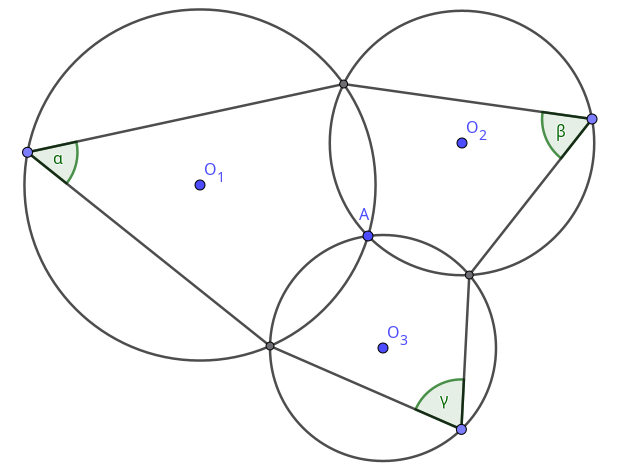
\includegraphics[scale=0.7]{ExK_1_1}}
	
\end{document}